\chapter{Introduction}
\label{ch:intro}
Hello, World!

\section{Motivation}
\label{sec:Motivation}
Iterative learning control (ILC), which operates the same task repeatedly and updates the control input according to the previous trial data, has been applied in tracking control applications for many years [\cite{ahn2007iterative}]. Since the learning operation can be non-casual, ILC has been shown to achieve better tracking performance compared to feedback control approaches [\cite{bristow2006survey}]. 


\begin{figure}
\begin{center}
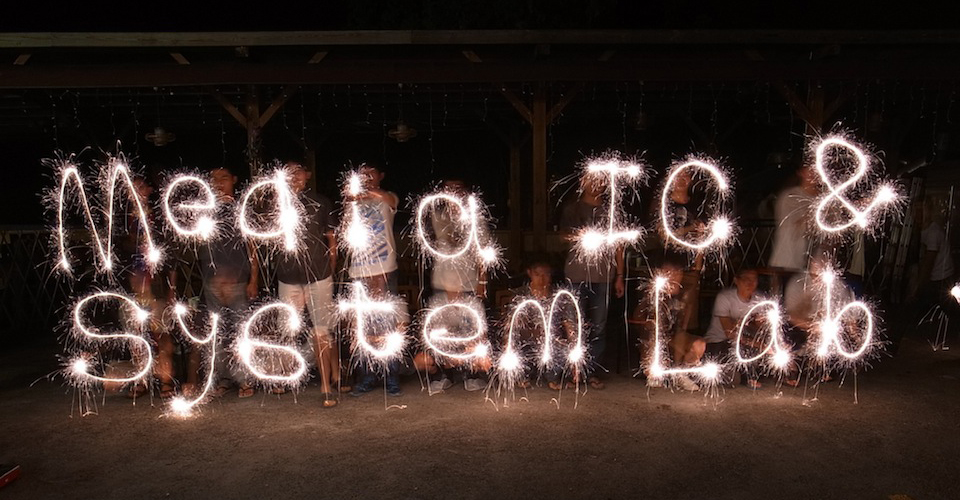
\includegraphics[width=0.8\linewidth]{inc/1_introduction/figure/misl.jpg}
\end{center}
\caption{
We are from Media IC \& System Lab.
}
\label{fig:misl}
\end{figure}


%\subsection{Table}
%\label{sec:Table}
%The related information is shown in~\tabref{lab_information}.
%
%\begin{table}[p]
%\vergap{0.8}
%\horgap{4.5pt}
%\caption{Lab information.}
%\vspace{5pt}
%\label{tab:lab_information}
%\centering
%\footnotesize 
%\begin{tabular}{cc}
%\toprule
%Property & Description \\
%\midrule
%Professor & Shao-Yi Chien \\
%Labs & BL421, MD431, MD726 \\
%\bottomrule
%\end{tabular}
%\end{table}


\section{Previous Work and Problem Formulation}
\label{sec:Previous Work and Problem Formulation}

To reduce the tracking error iteratively, the ILC updating law has to be well designed. The model-based ILC [\cite{lee1994feedback}; \cite{harte2005discrete}] uses the system inverse model as the learning filter to conduct the learning process. For these approaches, if the system model is identified accurately, the learning process would converge within few iterations [\cite{teng2015comparison}]. However, inversion-based methods require delicate modeling process in advance, which isn't practical for industry applications. Due to the reasons mentioned above, the development of model-free ILC becomes more and more popular in the ILC research community [\cite{janssens2011model}].

For the model-free approaches, the PD-type ILC [\cite{arimoto1984bettering}; \cite{chen2006pd}] is the simplest way to implement. However, monotonic convergence condition is not always satisfied by tuning the PD-parameters [\cite{moore2005monotonically}], and the tuning process may be time-consuming and damage the system. Time-reversal based ILC [\cite{ye2005zero}] uses the adjoint operator of the system as the learning filter, and the control updating law can be implemented by filtering the reversed error signals using the system itself. However, the learning rate of the time-reversal based ILC is usually slow [\cite{chen2017data}].  

To achieve a fast error convergence rate, the model-free inversion-based iterative learning control (MFIIC) [\cite{kim2012modeling}] applies the point-by-point division over the discrete frequency interval to estimate the system inverse dynamics from the input and output signals. Nevertheless, the output disturbances present in the denominator of the computation. Once unpredicted output disturbances are introduced, the magnitude of the denominator may approach to zero. This unpredicted phenomenon leads to a poor transient learning behavior [\cite{de2018improving}]. To improve the learning transient performance, NLIIC [\cite{de2019data}] uses an adaptive learning gain to avoid the division by a small numbers. However, since the adaptive learning gain shuts down the learning for the frequency components dominated by the output disturbances, the tracking performance in steady-state is degraded.      


\section{Proposed Approach and Contributions}
\label{sec:Proposed Approach and Contributions}

To overcome the difficulties mentioned above, a model-free learning algorithm is proposed. The proposed algorithm is based on the time-reversal based ILC, and we apply a data-based learning filter to update the control input every $n$ iterations. This approach not only accelerates the convergence rate of time-reversal based ILC. Compared to the MFIIC and NLIIC approaches, our method provides a more flexible updating law that gains the robustness against output disturbances and the tracking performance in steady-state.

\section{Thesis Overview}
\label{sec:Thesis Overview}

The remainder of this paper is organized as follows: Section 2 illustrates the basic iterative learning control algorithm and the existing model-free ILC approaches. Section 3 provides a derivation and analysis of the proposed model-free learning algorithm. Section 4 presents the simulation results to validate the effectiveness of the proposed algorithm. Finally, Section 5 summarizes the main results and contributions of this paper.